
% This LaTeX was auto-generated from MATLAB code.
% To make changes, update the MATLAB code and republish this document.

\documentclass{article}
\usepackage{graphicx}
\usepackage{color}

\sloppy
\definecolor{lightgray}{gray}{0.5}
\setlength{\parindent}{0pt}

\begin{document}

    
    \begin{verbatim}
function [] = Q4_20()
%  Solves the system of 1st order ODEs in question 4.20 %%%
%     Plots the result


% Define our constants
global L1 L2 L3 R1 R2

L1 = 5;
L2 = 8;
L3 = 6;

R1 = 100;
R2 = 150;


% Let's go

[TOUT,YOUT] = ode45(@dydtsys,[0, 5],[0; 0; 0]);

close all
figure
hold on
plot(TOUT,YOUT);
box on
grid on
xlabel('Time [s]')
ylabel('Current [A]')
legend('i_1','i_2','i_3')
title('Currents in Q4.20')
hold off


end



function idot = dydtsys(t,i)
% The function dydtsys is used to hold the ODEs
% t is the current time (a single number).
% i is a three element vector;
% i = [i1; i2; i3]
% idot is di/dt of each of these three variables

% Hard coding constants
global L1 L2 L3 R1 R2

i1 = i(1);
i2 = i(2);
i3 = i(3);

idot(1,1) = R1*(i2-i1)/L2;
idot(2,1) = (R1*(i1-i2) + R2*(i3-i2))/L1;
idot(3,1) = R2*(i2-i3)/L3 + 20*sin(6*t)/L3;

end
\end{verbatim}

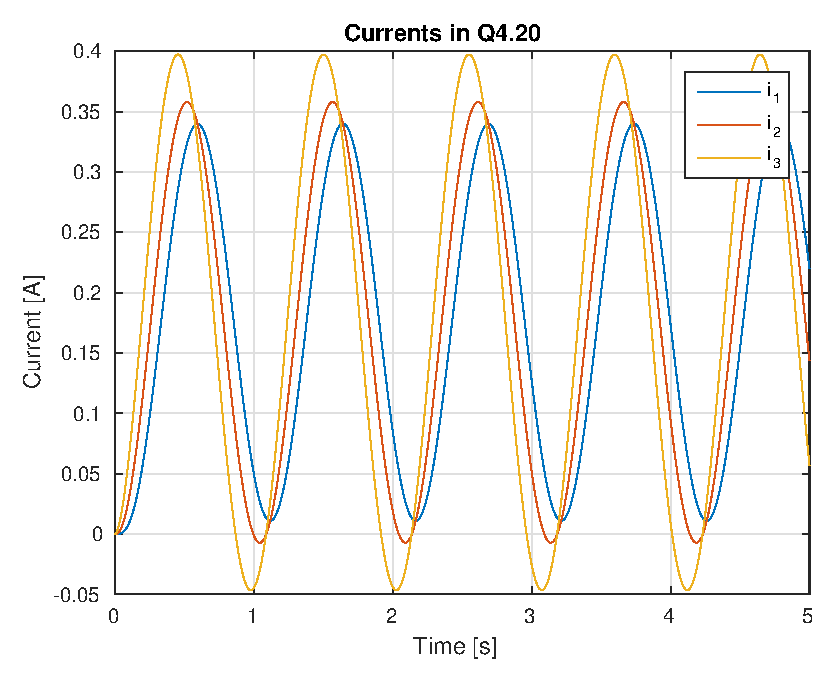
\includegraphics [width=4in]{Q4_20_01.eps}



\end{document}
    
